\chapter{Development Methodologies}

In order to achieve all the goals that this project has set out to achieve, a 
software development process will be required to be implemented and followed. 
The advantages of structuring such a software development project into a set of 
defined processes far outweighs the disadvantages \citep{knott_dawson99}. 

These defined processes form part of a process model, to which a process model 
can be described as:
\begin{itemize}
	\item a conquer and divide approach of problems into tasks at each stage;
	\item adding an element of control and planning;
	\item allowing for progress to be mapped visually;
	\item providing a structured approach to development;
	\item allowing for a higher quality of code and documentation to be produced.
\end{itemize}

The oldest formalised methodology for building software products was known as 
the systems development life cycle (SDLC) \citep{elliott04}. The SDLC
methodology utilises a structured and methodical approach, where by each stage 
of the life cycle is to be carried out rigidly and in order.

Within this chapter, various software development methodologies will be discussed 
and evaluated, ultimately leading to a software development methodology being 
chosen to use within this project.

% Waterfall Methodology
\newpage
\section{Waterfall}
A fundamental aspect to the waterfall model is the fact that the project is 
expected to progress down the primary path \citep{sergei:2012:Online}. The 
primary path is the most commonly used path through out a system. By 
highlighting the primary path, the major processes and tasks are easily mapped
out, a clear indication of what exactly is required to be completed.

The waterfall model contains six main phases --- requirements analysis, 
specification, design, coding, testing and implementation \citep{dawson09}. 
Deliverables are achieved as the flow down the primary path is completed. 

It is possible however for a reverse flow. This reverse flow represents a 
change applied to a prior deliverable, which was only recognised in the 
deliverable after the change is required in. This is known as rework, and can 
result in both the current deliverable and previous deliverables to be 
repeated.

\begin{figure}[H]
  \centering
  \vspace{-40pt}
  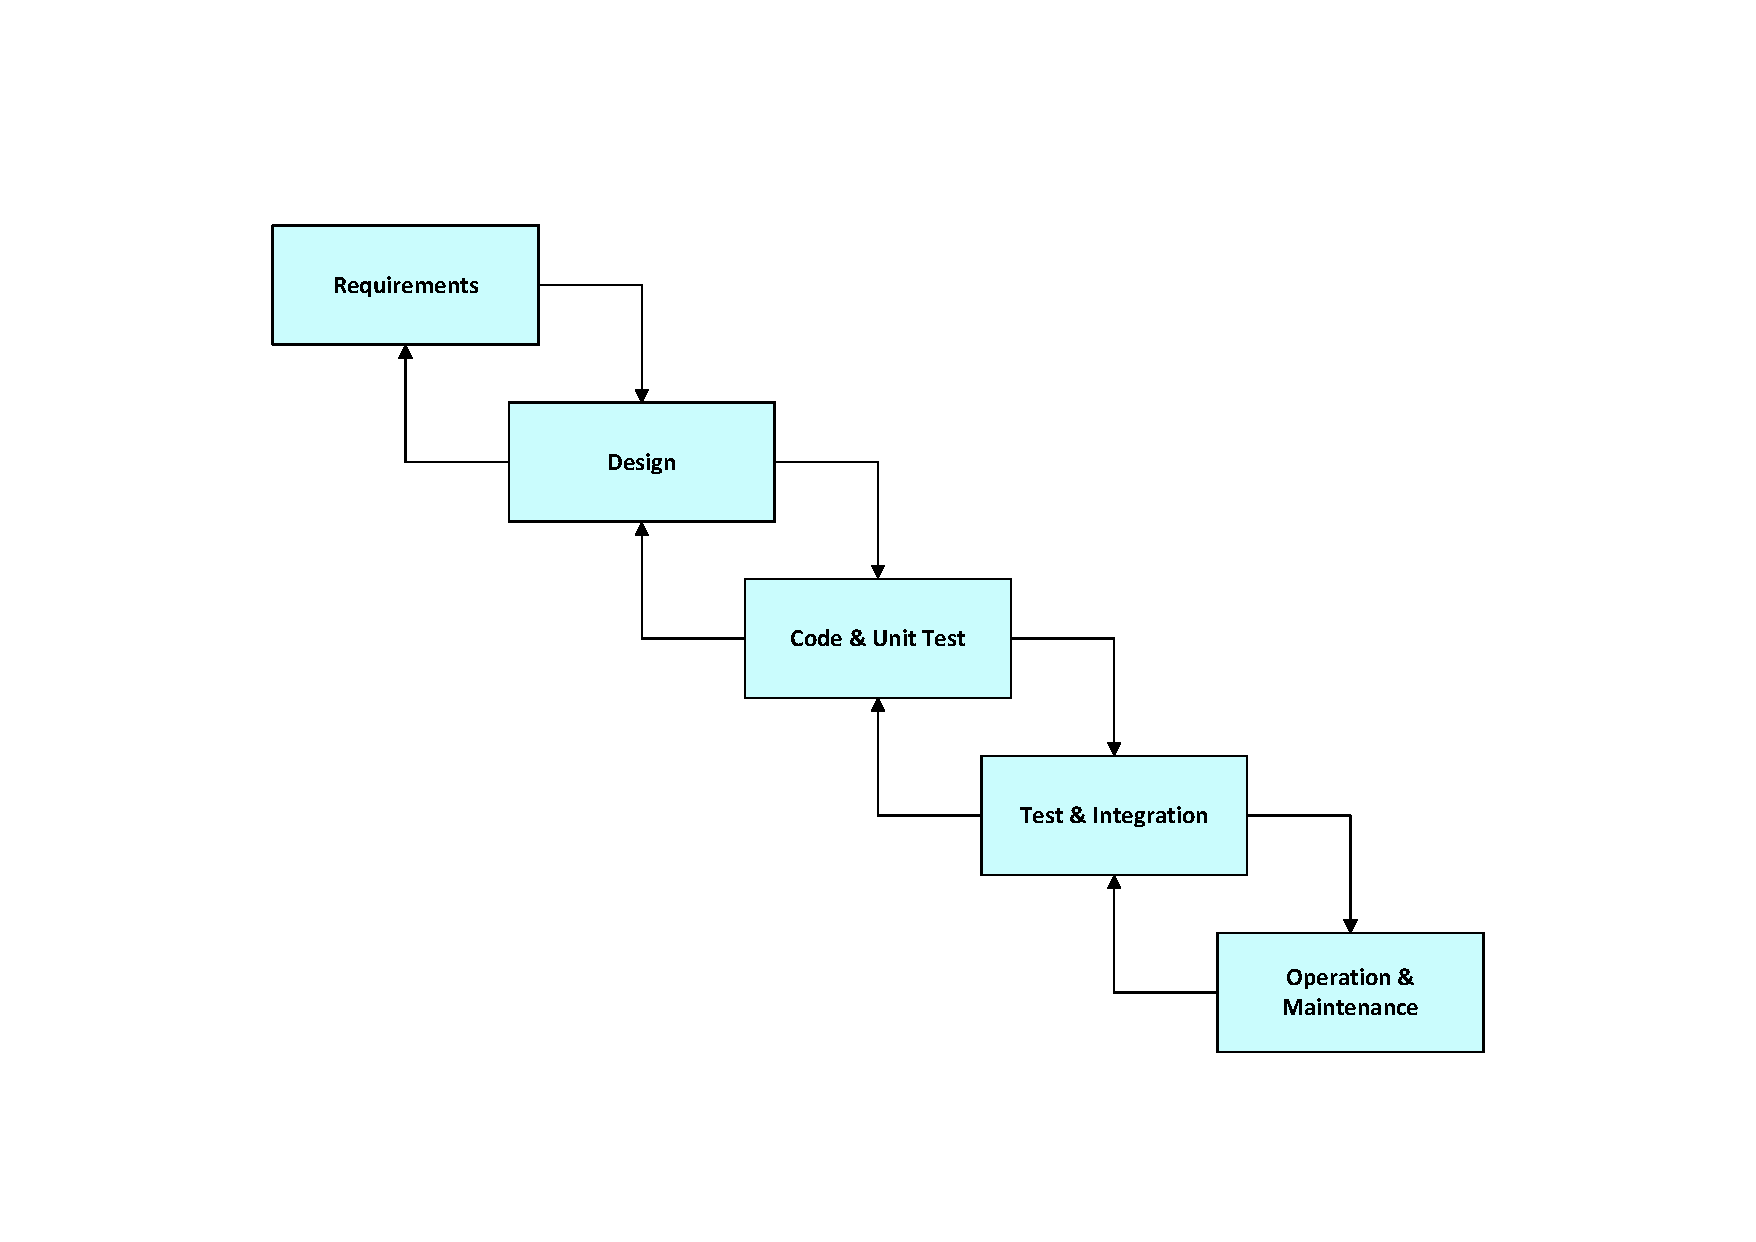
\includegraphics[width=\linewidth]{chapter6/waterfall.pdf}
  \vspace{-40pt}
    \caption[Waterfall methodology]
      {Waterfall methodology highlighting the ``flow'' through the various 
      sections that make up a software development project.}
\end{figure}

\subsection{Advantages}
The waterfall model is the most commonly used methodology due to the following 
reasons \citep{alam:2012:Online}:
\begin{itemize}
	\item Documentation is produced at every stage, allowing for anyone to join
        the project at any time to have full understanding;
  \item Minimum resources are required to implement this model, and is simple
        to implement and follow;
  \item Testing is completed after every major stage of software development.
\end{itemize}

\subsection{Disadvantages}
However, the disadvantages of this methodology are \citep{alam:2012:Online}:
\begin{itemize}
	\item The model works well if there is no reverse flow. Reverse flow can 
        cause time delays;
  \item The model assumes that the client know exactly what they want, in 
        reality this is not the case;
  \item A working model of the software is not complete, until the end product 
        has been finished.
\end{itemize}

% Incremental Methodology
\newpage
\section{Incremental}
The incremental software development methodology is an evolutionary extension 
of the waterfall model \citep{pressman09}. 

The main idea behind this development methodology is that developments are made
in increments, with each increment proving some additional functionality. This
additional functionality often only contains a small progression towards the 
final goal (or product).

Using an incremental approach allows the client to provide feedback, and thus 
the feedback be integrated into the product during development 
\citep{elliott04}. This incremental process continues until the final, 
completed product has been delivered. 

\begin{figure}[H]
  \centering
  %\vspace{-80pt}
  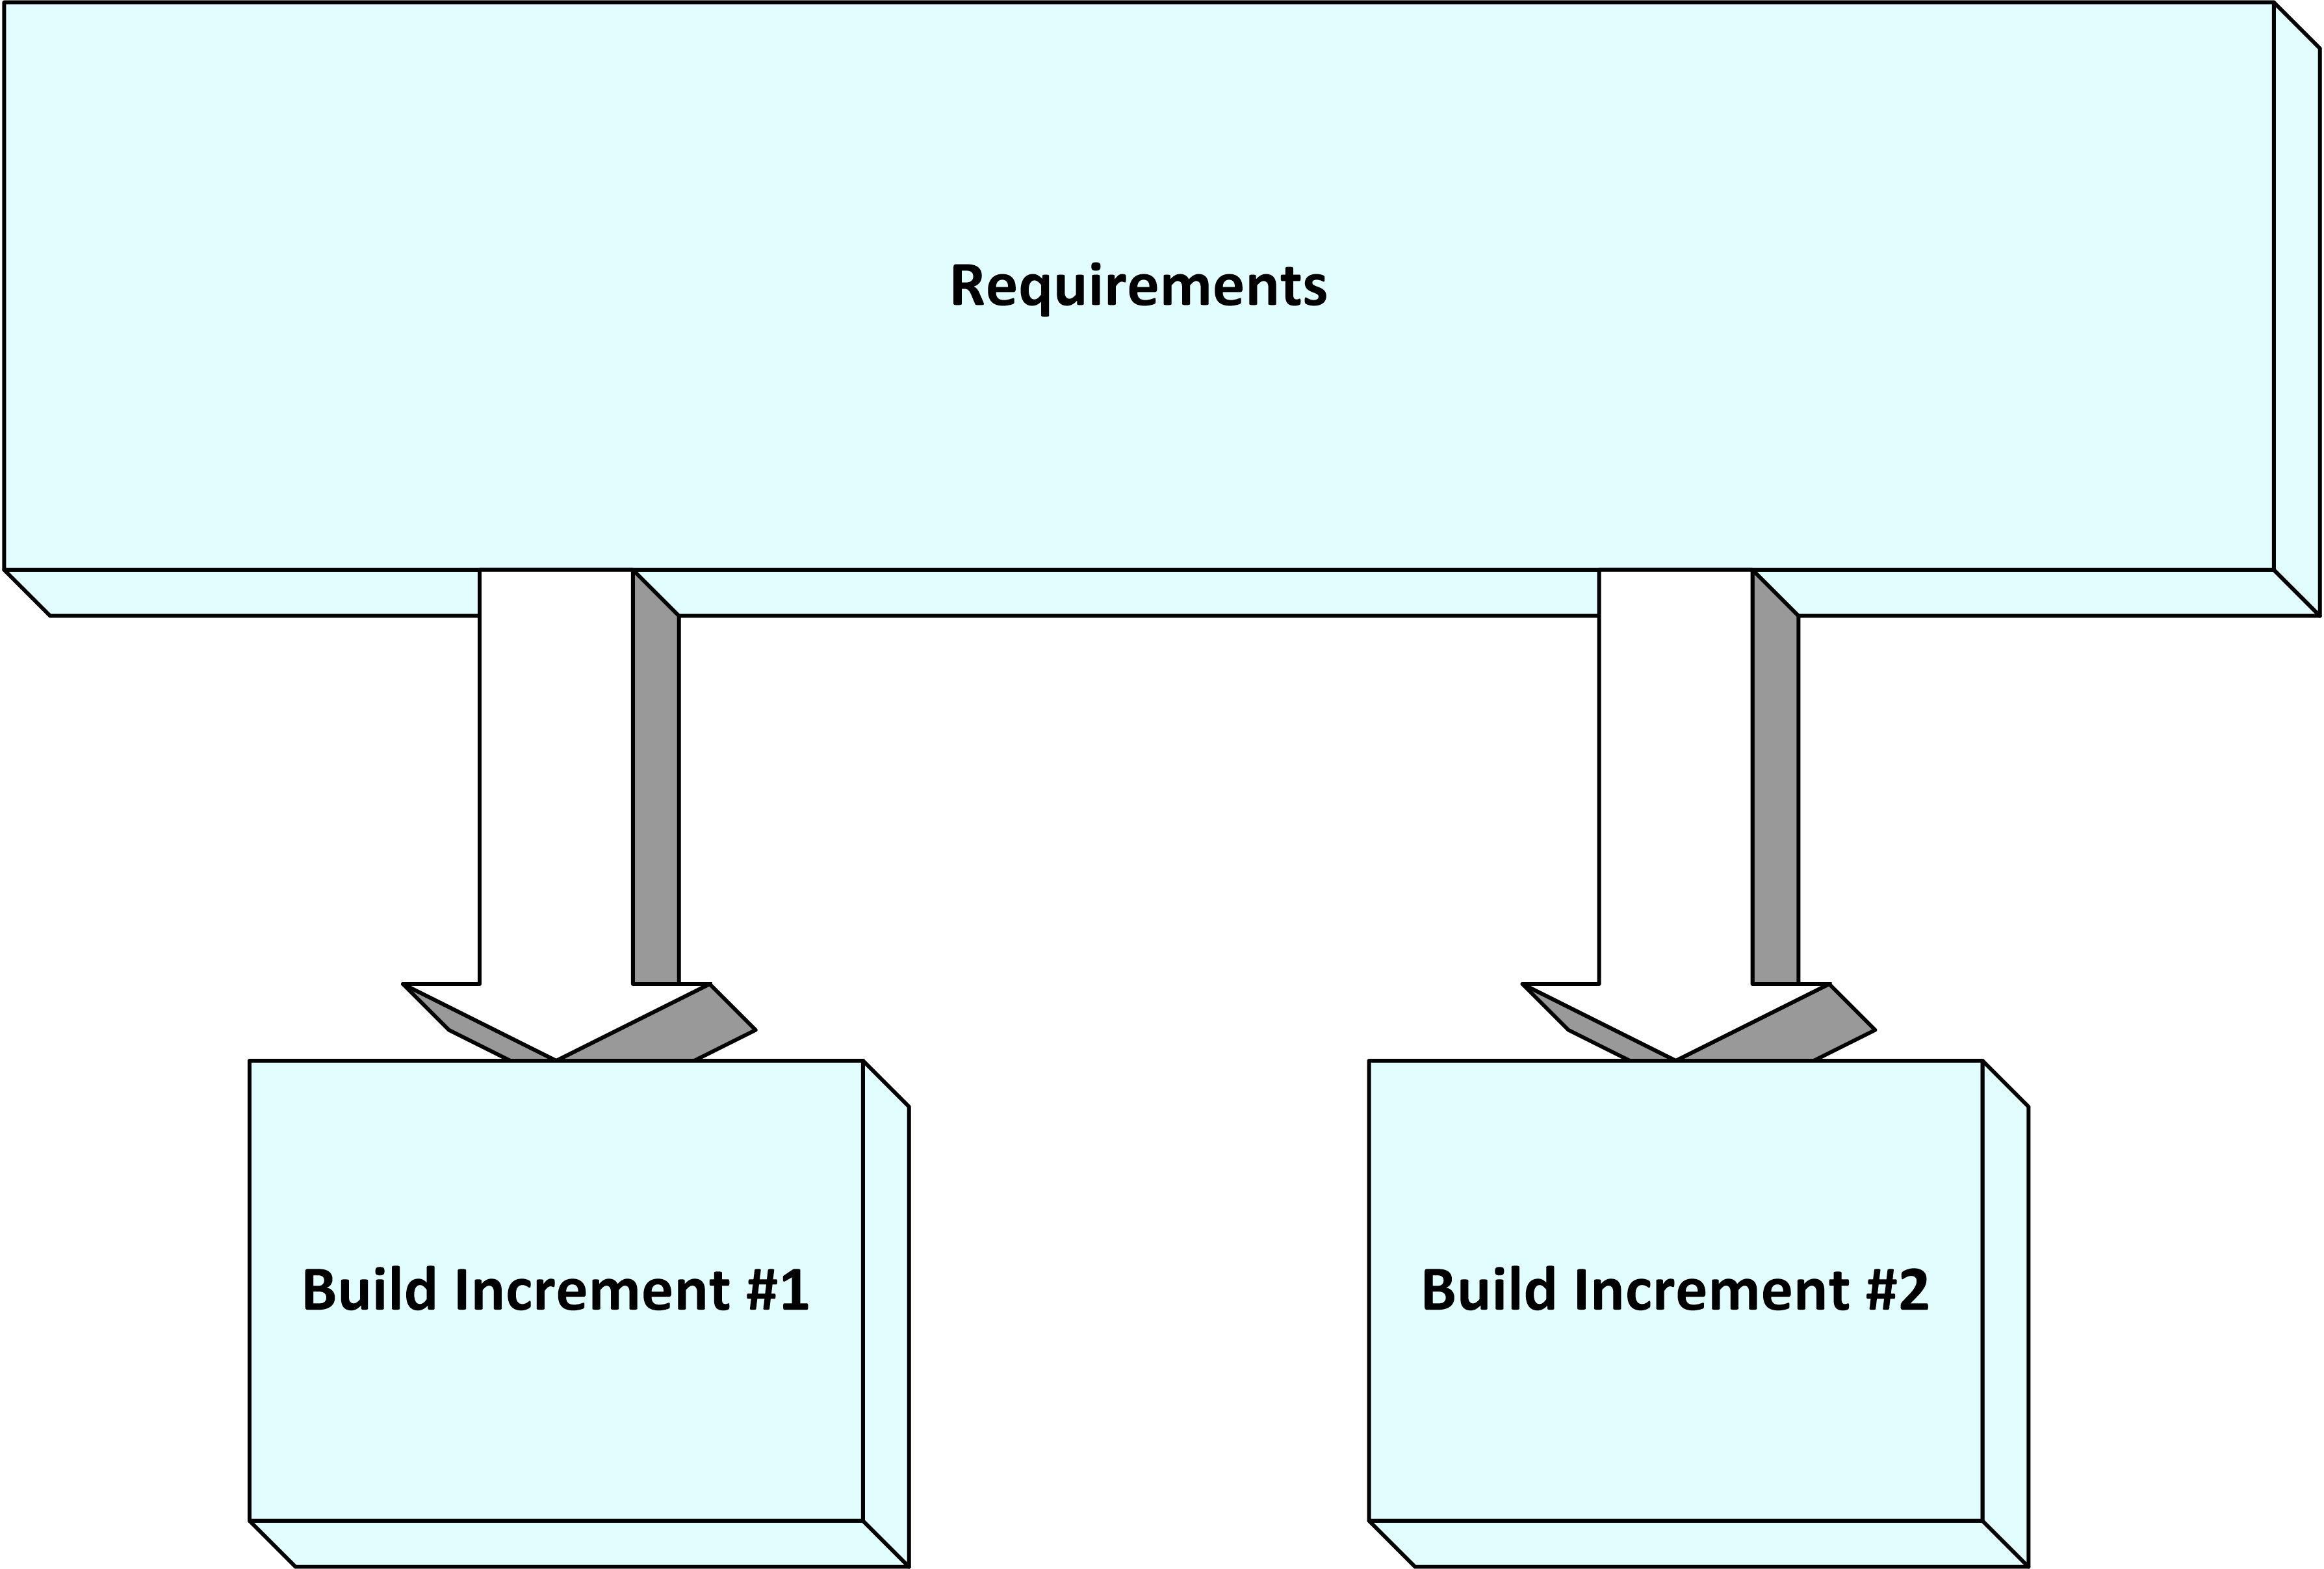
\includegraphics[scale=0.6]{chapter6/incremental.png}
  %\vspace{-60pt}
    \caption[Incremental methodology]
      {The incremental methodology allows for the requirements to be segmented 
      into an incremental series of the ``products''.}
\end{figure}

\subsection{Advantages}
The incremental software development methodology could be regarded as having 
the following advantages \citep{elliott04,SDT:2012:Online}:
\begin{itemize}
	\item The user is able to get an early idea of the system's capabilities;
	\item Early and continuous feedback is available from the client;
	\item It allows for more accurate planning, and slippage is easier to spot 
        due to the more frequent deadlines;
	\item It can be easier to test and debug, as any changes that are made within 
        an iteration are small;
	\item The user is able to learn how to use the system ``on the go'' rather 
        than in ``one go''.
\end{itemize}

\subsection{Disadvantages}
There are a number of disadvantages when utilising the incremental software 
development methodology \citep{elliott04,sergei:2012:Online}:
\begin{itemize}
	\item Development can occur for long periods of time, which might exceed the 
        original budget;
	\item Problems related to the system architecture could arise, if additional 
        functionality is added which was not 
				evident in earlier prototypes;
	\item The client may point out too many improvements, which would cause the 
        project to overrun or be completed not meeting the original 
        specification.
\end{itemize}

% Prototyping Methodology
\newpage
\section{Prototyping}
Prototyping is used when there is uncertainty about the technical solution to 
a problem \citep{dawson09}. 

It can be often useful to perform a number of experimental prototypes in order 
to gain understanding and knowledge, such as working on a new hardware platform
or developing a new algorithm. 

The prototyping software development methodology allows for many ideas and 
theories to be implemented, tested and evaluated. There are two main forms of 
prototyping, throw-away prototyping and evolutionary prototyping.

\subsection{Throw-away prototyping}
Once a prototype has been developed, the product associated with the prototype 
could be thrown away, with the actual development of the desired product 
starting from a blank ``canvas''.

\subsubsection{Advantages}
\citet{knott_dawson99} mention the following list of advantages over other 
software development methodologies: 
\begin{itemize}
  \item Errors and omissions in the requirements specification can be quickly 
        fixed;
  \item An artificial is produced quickly (keeping the client happy);
  \item The prototype is able to test the feasibility of the product;
  \item Alternatives of a various prototypes can be compared;
  \item Allows for improvement of communication between the developer and the 
        client.
\end{itemize}

\subsubsection{Disadvantages}
\citet{dawson09} highlights that there are a number of issues with the 
throw-away prototyping methodology, as highlighted below:
\begin{itemize}
  \item The prototype may contain a number of bugs;
  \item The prototype might look good, but technically could be poor. If it was 
        integrated into the system, then this could lead to poorly structured 
        code.
  \item Prototype development within a different language or system to the 
        final implementation may allow for technical differences to occur.
\end{itemize}

\subsection{Evolutionary prototyping}
Unlike the throw-away prototyping, a prototype could be developed further into
the final desired product. Utilising this idea, is known as evolutionary 
prototyping.

\subsubsection{Advantages}
The advantages are generally the same as the advantages found within the 
throw-away prototyping methodology with the following addition:
\begin{itemize}
  \item Any code that is developed, is reused and improved.
\end{itemize}

\subsubsection{Disadvantages}
As with the advantages, the disadvantages are generally the same as the 
advantages found within the throw-away prototyping methodology with the 
following addition:
\begin{itemize}
  \item A well structured design of code is required so that it can be 
        developed and allow for the evolution process to occur.
\end{itemize}

% Agile Methodology
\newpage
\section{Agile}

The agile software development methodology is designed to "reduce risk by 
delivering software systems in short bursts or releases" \citep{dawson09}. 

The concept behind the agile software development is to reduce the total weight
time that clients have to endure, by releasing working systems in as little 
time as possible. 

Each iteration may not contain a full working system, but it will contain a 
partial system, that could be used by the client. Agile methods are suited to 
projects that have unclear or rapidly changing requirements \citep{dawson09}.

\subsection{Advantages}
\citet{dawson09} states that the main principles of the agile software 
development methodology is as follows:

\begin{itemize}
	\item The methodology surrounds the concept of regular face-to-face meetings
        (as opposed to in-depth documentation);
	\item A close working relationship between the client and the developers;
	\item A short iterative time scale (usually weeks rather than months or 
        years);
	\item Easily able to change the requirements at any stage.
\end{itemize}

\subsection{Disadvantages}
However, \citet{dawson09} also states that the agile software development 
methodology does have it's problems:
\begin{itemize}
	\item There can be a limited amount of documentation, as this step is usually 
        skipped to save time;
  \item The uncertainty of a specification may lead to poor code and/or 
        structure.
\end{itemize}

% Extreme Programming Methodology
\newpage
\section{Extreme Programming}
Extreme Programming is a software development methodology intended to improve 
upon the agile methodology. It attempts to do this by maintaining high software 
quality whilst also maintaining high responsiveness to changing client 
requirements \citep{knott_dawson99}.

As found in agile development, there are many frequent release, and development 
is completed in short cycles, intended to improve productivity and to introduce 
check points (client requirements can be changed).

\subsection{Advantages}
The extreme programming software development methodology shares the same 
advantages as the agile and the evolutionary prototyping methodologies.

\subsection{Disadvantages}
As with the advantages, the disadvantages of the extreme programming methodology 
are shared amongst the agile and the evolutionary prototyping methodologies.

% Summary
\newpage
\section{Summary}
In order to achieve the best product possible, it is clearly evident that the 
client must be kept in the loophole as often as possible. This allows for any 
revisions, modifications, and changes to be considered and implemented with as 
little delay as possible.

Although this project has some well defined requirements, the details of the 
requirements are incomplete in some areas. However some key details have 
already been set, such as the programming language to be used and the target 
system. 

The rule of thumb states that if uncertainty is high then the use of an 
evolutionary approach is recommended \citep{hughes_cotterell09}. As well as 
this, the incremental approach seems to be an ideal methodology to utilise. 
The incremental methodology is ideal for projects that have a tight schedule 
\citet{hughes_cotterell09}.

Although the schedule of the project is not necessarily tight, it does contain 
a lot of potentially time consuming design research. By utilising the 
incremental methodology as a fundamental methodology, this should allow for 
small incremental developments to occur, with little work to re-complete if the
original path is later deemed to be incorrect.

Within each increment, an evolutionary prototype approach will be taken. The 
main reason for this is that it allows for development and research to coexist 
side by side. If the research pays off, then it's output can directly be 
utilised within the final published product.